\documentclass[]{book}
\usepackage{lmodern}
\usepackage{amssymb,amsmath}
\usepackage{ifxetex,ifluatex}
\usepackage{fixltx2e} % provides \textsubscript
\ifnum 0\ifxetex 1\fi\ifluatex 1\fi=0 % if pdftex
  \usepackage[T1]{fontenc}
  \usepackage[utf8]{inputenc}
\else % if luatex or xelatex
  \ifxetex
    \usepackage{mathspec}
  \else
    \usepackage{fontspec}
  \fi
  \defaultfontfeatures{Ligatures=TeX,Scale=MatchLowercase}
\fi
% use upquote if available, for straight quotes in verbatim environments
\IfFileExists{upquote.sty}{\usepackage{upquote}}{}
% use microtype if available
\IfFileExists{microtype.sty}{%
\usepackage{microtype}
\UseMicrotypeSet[protrusion]{basicmath} % disable protrusion for tt fonts
}{}
\usepackage[margin=1in]{geometry}
\usepackage{hyperref}
\hypersetup{unicode=true,
            pdftitle={MTXQCvX2 documentation},
            pdfauthor={Christin Zasada},
            pdfborder={0 0 0},
            breaklinks=true}
\urlstyle{same}  % don't use monospace font for urls
\usepackage{natbib}
\bibliographystyle{apalike}
\usepackage{longtable,booktabs}
\usepackage{graphicx,grffile}
\makeatletter
\def\maxwidth{\ifdim\Gin@nat@width>\linewidth\linewidth\else\Gin@nat@width\fi}
\def\maxheight{\ifdim\Gin@nat@height>\textheight\textheight\else\Gin@nat@height\fi}
\makeatother
% Scale images if necessary, so that they will not overflow the page
% margins by default, and it is still possible to overwrite the defaults
% using explicit options in \includegraphics[width, height, ...]{}
\setkeys{Gin}{width=\maxwidth,height=\maxheight,keepaspectratio}
\IfFileExists{parskip.sty}{%
\usepackage{parskip}
}{% else
\setlength{\parindent}{0pt}
\setlength{\parskip}{6pt plus 2pt minus 1pt}
}
\setlength{\emergencystretch}{3em}  % prevent overfull lines
\providecommand{\tightlist}{%
  \setlength{\itemsep}{0pt}\setlength{\parskip}{0pt}}
\setcounter{secnumdepth}{5}
% Redefines (sub)paragraphs to behave more like sections
\ifx\paragraph\undefined\else
\let\oldparagraph\paragraph
\renewcommand{\paragraph}[1]{\oldparagraph{#1}\mbox{}}
\fi
\ifx\subparagraph\undefined\else
\let\oldsubparagraph\subparagraph
\renewcommand{\subparagraph}[1]{\oldsubparagraph{#1}\mbox{}}
\fi

%%% Use protect on footnotes to avoid problems with footnotes in titles
\let\rmarkdownfootnote\footnote%
\def\footnote{\protect\rmarkdownfootnote}

%%% Change title format to be more compact
\usepackage{titling}

% Create subtitle command for use in maketitle
\newcommand{\subtitle}[1]{
  \posttitle{
    \begin{center}\large#1\end{center}
    }
}

\setlength{\droptitle}{-2em}

  \title{MTXQCvX2 documentation}
    \pretitle{\vspace{\droptitle}\centering\huge}
  \posttitle{\par}
    \author{Christin Zasada}
    \preauthor{\centering\large\emph}
  \postauthor{\par}
      \predate{\centering\large\emph}
  \postdate{\par}
    \date{2019-02-09}

\usepackage{booktabs}
\usepackage{longtable}

\ifxetex
  \usepackage{letltxmacro}
  \setlength{\XeTeXLinkMargin}{1pt}
  \LetLtxMacro\SavedIncludeGraphics\includegraphics
  \def\includegraphics#1#{% #1 catches optional stuff (star/opt. arg.)
    \IncludeGraphicsAux{#1}%
  }%
  \newcommand*{\IncludeGraphicsAux}[2]{%
    \XeTeXLinkBox{%
      \SavedIncludeGraphics#1{#2}%
    }%
  }%
\fi
\usepackage{booktabs}
\usepackage{longtable}
\usepackage{array}
\usepackage{multirow}
\usepackage[table]{xcolor}
\usepackage{wrapfig}
\usepackage{float}
\usepackage{colortbl}
\usepackage{pdflscape}
\usepackage{tabu}
\usepackage{threeparttable}
\usepackage{threeparttablex}
\usepackage[normalem]{ulem}
\usepackage{makecell}

\usepackage{amsthm}
\newtheorem{theorem}{Theorem}[chapter]
\newtheorem{lemma}{Lemma}[chapter]
\theoremstyle{definition}
\newtheorem{definition}{Definition}[chapter]
\newtheorem{corollary}{Corollary}[chapter]
\newtheorem{proposition}{Proposition}[chapter]
\theoremstyle{definition}
\newtheorem{example}{Example}[chapter]
\theoremstyle{definition}
\newtheorem{exercise}{Exercise}[chapter]
\theoremstyle{remark}
\newtheorem*{remark}{Remark}
\newtheorem*{solution}{Solution}
\begin{document}
\maketitle

{
\setcounter{tocdepth}{1}
\tableofcontents
}
\chapter{Welcome}\label{welcome}

Let's get started \ldots{}. this part is going to be written in the
proximate future.

\chapter{Introduction MTXQCvX documentation}\label{intro}

This documentation introduces to you how to use MTXQCvX2 in order to run
a first straight-forward data analysis of your metabolomics experiment.
The underling experimental and mathematical concepts have been
introduced for the pulsed stable isotope resolved metabolomics (pSIRM)
approach published in \citep{Pietzke2014}.

This documentation shows you how to use MTXQCvX2 in order to assess the
quality of your GC-MS derived data, perform the determination of
calibration curves and absolute quantification. It furthermore provides
you two normalisation strategies and the calculation of quantities in,
e.g., pmol/1e+6 cells or pmol/mg tissue.

MTXQCvX2 does also enable the calculation of stable isotopic
incorporation and the evaluation of the underlying data, the mass
isotopomer distributions (MIDs).

The tool has been set up to support the in-lab developed workflow for
quantitative metabolomics experiments using the in-house developed
software Maui for the annotation of data. MTXQCvX2 bridges the gap
between quality control and first data post-processing / analysis of
GC-MS derived data (MTXQCvX2\_part1, MTXQCvX2\_part2).

Nevertheless MTXQCvX2 includes a module in order to integrate all kind
of data provided in spreadsheet-format, e.g., derived from metmax,
extracting required information and creating corresponding files
(MTXQCvX2\_part4).

\section{Structure}\label{structure}

MTXQCvX2 contains a suite of modules is optimized to process GC-MS
derived data and processed either in Maui or Chromatof/Metmax. Workflows
for both approaches are introduced with step-by-step instructions in
chapter @\ref(maui) and @\ref(metmax).

Subsequently each MTXQCvX2 module (chapter \ref{ExpSetup} -
\ref{Metmax}) is introduced in greater detail including a input / output
files and processing parameter.

The configuration of MTXQCvX2 has been split into two categories - (1) a
general configuration \texttt{config\_files} and (2) metabolomics
specific parameters \texttt{config\_mtx}. Latter one is meant to provide
flexibility including further substances. How to do so and what files
can be customizes is shown in chapter \ref{config}.

Workflow-specific processing methods applied in Chromatof are introduced
separately in the chapter \ref{mauiproc} and \ref{metmaxproc} including
all parameter as well as a short introduction.

The remaining chapter cover a chapter for frequently asked questions
(chapter\ref{FAQ}) that might give you a hint where to search for the
information you are looking for.

The appendix summarises technical reference material in the form of a
dictionary of tables (chapter \ref{tables}), protocols for the pSIRM
workflow \ref{psirm} and a complete distinct chapter listing protocols
(chapter \ref{protocols}) including standard and sample preparation and
derivatisation (chapter \ref{SampleExtraction} and \ref{Deriv}) and the
current setting of the GC-ToF-MS machine (chapter \ref{gcms}).

\section{How to use this
documentation}\label{how-to-use-this-documentation}

This documentation provides for each level the right starting point.
Complete newbies are highly suggested to start with one of the two
tutorials and following the step-by-step descriptions using the example
datasets. Also if you are using for the first time please go through to
the chapter once to be aware of all the steps that are required to
succeed.

Experienced users might be referred to the explanation of the individual
modules or to the how-to-guides for data processing and the FAQs
section.

\section{Example datasets and files}\label{example-datasets-and-files}

introduce inst/template folder

\section{\texorpdfstring{\texttt{What\ do\ I\ do\ if\ I\ don\textquotesingle{}t\ find\ the\ answer?}}{What do I do if I don't find the answer?}}\label{what-do-i-do-if-i-dont-find-the-answer}

If you are familiar with github and the create an issue - please head on
to the gihub repository (github.com/ChrisZasa/MTXQC\_documentation) of
this documentation and create one or write me a message.

\chapter{Tutorial: Maui-annotation projects}\label{maui}

\section{Read this in case}\label{read-this-in-case}

\begin{itemize}
\tightlist
\item
  you have successfully finished the annotation using Maui-SILVIA
\item
  exported all required MAUI container (see \ref{mauiexport})
\item
  you have a list of your GC-MS sequence and related experimental
  conditions
\item
  you know the extraction procedure of standards and samples
\end{itemize}

\section{In a nutshell}\label{nutshellmaui}

\begin{enumerate}
\def\labelenumi{\arabic{enumi}.}
\tightlist
\item
  Setup a new R-project
\item
  Copy all MTXQC template files and folders
\item
  \emph{Knit with parameter}: \texttt{MTXQC\_init.Rmd} and create
  project folder (e.g., \texttt{psirm\_glucose})
\item
  Copy input files and rename \texttt{ManualQuantTable.tsv}
  (e18205cz.tsv)
\item
  Create your \texttt{annotation.csv} and \texttt{sample\_extracts.csv}
  files
\item
  Define the internal extraction standard
\item
  \emph{Knit with parameter}: \texttt{MTXQC\_ExperimentalSetup.Rmd}
\item
  \emph{Knit with parameter}: \texttt{MTXQC\_part1.Rmd}
\item
  \emph{Knit with parameter}: \texttt{MTXQC\_part2.Rmd}
\item
  If required, proceed with \texttt{MTXQC\_part3.Rmd} for manual
  validation of your data
\end{enumerate}

\section{\texorpdfstring{Dataset of the tutorial -
\texttt{tutorial\_single\_maui}}{Dataset of the tutorial - tutorial\_single\_maui}}\label{dataset-of-the-tutorial---tutorial_single_maui}

Copy the dataset \texttt{tutorial\_single\_maui} somewhere local on your
computer or laptop. The dataset represents the data of the first psirm
metabolomics experiment in the Kempa Lab. HEK293 cells have been
cultivated at 21\% oxygen and a range of glucose levels (0.3 - 4.5 g/L
Glc) and constant glutamine concentration (4 mM) following standard cell
culture procedures. During the cell harvest cells have been labeled for
two minutes with uniformly labeled 13C-glucose, three replicates per
condition.

\section{In detail}\label{in-detail}

\subsection{Setup a R-project}\label{setup-a-r-project}

R-projects provide a secure environment to handle your data from the
processing in MTXQCvX2 until the final reports and analysis. Think about
it as a big bubble containing and carrying all your data and analysis
savely from one place to the other undisturbed of the outside changes.

\begin{itemize}
\tightlist
\item
  Open R-studio and create a new project following:
  \texttt{File\ -\textgreater{}\ New\ project\ -\textgreater{}\ New\ Project\ -\textgreater{}\ New\ Directory}
  and call the directory \texttt{tutorial\_single\_maui} and the
  preferred subdirectory.
\item
  I recommend to start each project in a new session (tick the box at
  the bottom of the dialogue box).
\end{itemize}

\subsection{Copy MTXQCvX2 template
files}\label{copy-mtxqcvx2-template-files}

\begin{itemize}
\tightlist
\item
  Download the current version of MTXQCvX2 called fluffy adventure
  \href{github.com/ChrisZasada/fluffy_adventure}{here}
\item
  Open and extract the zip-file
\item
  Copy all folders and files into your newly created R-project
  'tutorial\_single\_maui`
\end{itemize}

\subsection{\texorpdfstring{Process
\texttt{MTXQC\_init.Rmd}}{Process MTXQC\_init.Rmd}}\label{process-mtxqc_init.rmd}

The module \texttt{MTXQC\_init.Rmd} provides you two important things:
(1) Check-up package installation (2) Creation of project-folder

The project folder is supposed to provide a tidy structure while data
processing and analysis and contains several pre-defined folder. Besides
the following folders: `input', `output' and `figures' you see a
detailed subfolder structure. You find more details about each folder
and additional suggestion how to use project-folder in chapter
\ref{init}.

All you need to do is to process the \texttt{MTXQC\_init.Rmd}. The
following procedure is how you process all \texttt{.Rmd}-files of
MTXQCvX2:

\begin{itemize}
\tightlist
\item
  Click on the small black triangle next to the ball of yarn
\item
  Choose \texttt{Knit\ with\ Parameters...}
\end{itemize}

If the \texttt{.Rmd}-file contains defined parameters a shiny dialogue
pops up and provides an interactive selection based on the document. In
the case of \texttt{MTXQC\_init.Rmd} you are asked to define a so-called
project-folder, e.g., \texttt{psirm\_glucose}.

\begin{itemize}
\tightlist
\item
  Define the name of the project-folder: \texttt{psirm\_glucose}
\end{itemize}

Check in the files tab of R-Studio if you see the new folder and browse
through it.

\subsection{Prepare and copy input
files}\label{prepare-and-copy-input-files}

Several files have to be exported from Maui and copied into the folders
\texttt{input/gc}, \texttt{input/quant} and \texttt{input/inc} for the
evaluation of the GC-MS performance, absolute quantification and isotope
incorporation.

Please follow the detailed instructions in section \ref{mauiexport} if
you need further information how to perform the export in Maui. For the
purpose of the tutorial the exported files are already processed and
copied into the corresponding subfolders of the \texttt{input}-folder.

\subsection{\texorpdfstring{Copy files: \texttt{annotation.csv} and
\texttt{Sample\_extracts.csv}}{Copy files: annotation.csv and Sample\_extracts.csv}}\label{copy-files-annotation.csv-and-sample_extracts.csv}

Both files contain important information about your metabolomics
experiment and since these information are highly specific you need to
create them on your own and save them in \texttt{project-folder/input/}.

Browse to both files in the tutorial dataset, have a look at the content
and copy both files into \texttt{psirm\_glucose/input}.

The herein shown \emph{annotation file} contains information about the
eperimental conditions of each sample and measurement file. The columns
\textbf{File} and \textbf{Type} are mandatory, additional columns
defining further parameter, like cell line or glucose level, are totally
customizable to your needs.

The \emph{sample extracts} file specify the nature and volume / weight
of the sample extracts. The columns \textbf{Extract\_vol} and
\textbf{Unit} are mandatory here. This file here shows cell extracts
defined with the unit \emph{count} for specific conditions. Please be
aware that names of experimental conditions have to match between
annotation and sample extracts file.

Nevertheless it is not necessarily required to define for each
combination of conditions a cell count. Please refer FAQs section
\ref{createannotation} and \ref{createsampleextracts} for further
information how to create and set up both files from the scretch.

\subsection{Define an internal standard - cinnamic
acid}\label{define-an-internal-standard---cinnamic-acid}

We have to define the internal extraction standard for each experiment
in \texttt{config\_mtx/conversion\_metabolite.csv}. Classical pSIRM
experiments like the one we are using for this tutorial used cinnamic
acid for tracking variations in experimental handling. This provides
flexibility in the experimental setup.

\begin{itemize}
\tightlist
\item
  Open the file: 'config\_mtx/conversion\_metabolite.csv`
\item
  Scroll down to the entry \texttt{Cinnamic\ acid\ trans-,\ 1TMS}
\item
  Define \texttt{InternalStandard} in the column \texttt{Standard}
\item
  Save the file and close it
\end{itemize}

\subsection{\texorpdfstring{Process
\texttt{MTXQC\_ExperimentalSetup.csv}}{Process MTXQC\_ExperimentalSetup.csv}}\label{process-mtxqc_experimentalsetup.csv}

\subsection{\texorpdfstring{Process
\texttt{MTXQC\_part1.Rmd}}{Process MTXQC\_part1.Rmd}}\label{process-mtxqc_part1.rmd}

\subsection{\texorpdfstring{Process
\texttt{MTXQC\_part2.Rmd}}{Process MTXQC\_part2.Rmd}}\label{process-mtxqc_part2.rmd}

\chapter{Workflow for Metmax-extracted projects}\label{wf:metmax}

\section{You want to follow this
\ldots{}}\label{you-want-to-follow-this}

\begin{itemize}
\tightlist
\item
  in case you have measured samples and quantification standards by
  GC-MS
\item
  performed the annotation of intermediates in ChromaToF or vendor
  software
\item
  exported all information into \texttt{.txt} files
\item
  used metmax to extract peak areas / mass isotopomer distributions
  (MIDs)
\end{itemize}

\section{Introduction}\label{introduction}

This document describes how to use MTXQCvX2 in combination with
metmax\footnote{\url{http://gmd.mpimp-golm.mpg.de/apps/metmax/default.htm}}.

Historically, MTXQCvX2 has been developed and optimized for Maui-derived
input files. The \texttt{MTXQCvX2-part4.Rmd} functions as a converter of
metmax-derived files in order to create suitable input formats for
\texttt{MTXQCvX-part1.Rmd}.

This module could also be used to convert tables derived from other
programs as long as they are stick with the herein described table
formats. Mandatory columns are referenced in the text for each kind of
input file.

The general workflow of the NMTXQCvX2 project is briefly shown below in
quick view. More detailed instructions are summarised in the following
paragraphs.

For more detailed explanations about the individual input parameter for
each module of MTXQCvX2 please proceed to read the documentation about
the individual modules and their knitting parameter. The relation of
knitting parameter, input and output files are described in each
section.

\section{Quick view}\label{quick-view}

\begin{enumerate}
\def\labelenumi{\arabic{enumi}.}
\tightlist
\item
  Generate input files: run \texttt{MTXQC\_part4.Rmd}\footnote{read here
    the instructions}
\item
  Setup R-project and copy MTXQC-files
\item
  Knit with parameter: \texttt{MTXQC\_init.Rmd}
\item
  Copy input files into corresponding folders
\item
  Create annotation.csv and sample\_extracts.csv files\footnote{Details
    further down this document}
\item
  Update metabolite names in
  \texttt{conversion\_metabolite.csv}\footnote{Column:
    Metabolite\_manual}
\item
  Define the internal standard and/or alkanes\footnote{Also in
    conversion\_metabolite.csv; see below paragraph Standards}
\item
  Knit with parameter: \texttt{MTXQC\_ExperimentalSetup.Rmd}
\item
  Knit with parameter: \texttt{MTXQC\_part1.Rmd}
\item
  Knit with parameter: \texttt{MTXQC\_part2.Rmd}
\item
  If required - proceed with \texttt{MTXQC\_part3.Rmd} for
  ManualValidation
\end{enumerate}

\section{Input files}\label{input-files}

If you need an introduction about how to use metmax - have a look at the
separate documentation \texttt{Metmax\_intro}.

The chapter \ref{part4} \texttt{MTXQCvX\_part4} explains in detail how
to use this module to generate suitable input files.

\section{Annotation-file}\label{annotation-file}

The annotation file relate file names with experimental conditions or
specify quantification standards in your batch. Two columns -
\textbf{File and Type} - are obligatory and have to be present in the
annotation file. In the case of their absence
\texttt{MTXQCvX\_part1.Rmd} stops processing and shows an error message.

A quick way to generate an annotation file is described below:

\begin{enumerate}
\def\labelenumi{\arabic{enumi}.}
\tightlist
\item
  Copy all file names from a file of your choice
\item
  Paste \& transpose the content into a new Excel-File into column A
\item
  Call column A -\textgreater{} File
\item
  Optional: Remove any non-file name entry in this column
\item
  Add the column Type and specify each file either as \textbf{sample},
  \textbf{Q1\_diluation}, ,\textbf{addQ1\_dilution}\footnote{see for
    further details additionalQuant}
\item
  Add more columns specifying your experimental conditions, e.g.,
  Cellline and Treatment\footnote{optimal: two-three parameter, max:
    four parameter. Consider possible combinations, e.g.,
    HCT116-control, HCT116-BPTES}
\item
  Save the content as \texttt{csv-file} in the
  \texttt{psirm\_glucose/input/...}
\end{enumerate}

\section{Sample\_extracts-file}\label{sample_extracts-file}

The \texttt{sample\_extracts.csv} file is required in order to determine
automatically absolute quantities in the manner of pmol/1e+6 cells or
pmol/mg tissue in the \texttt{CalculationFileData.csv}.

This file requires two obligatory columns - \textbf{Extract\_vol} and
\textbf{Unit}\footnote{Define: count, mg or ul}. Please specify for each
experimental condition the amount of extracted cells (count), tissue
(mg) or volume of blood/plasme (ul) in the unit shown in the brackets.\\
The names of the columns of the experimental conditions have to match up
with the annotation file. Save the file in the folder
\texttt{psirm\_glucose/input/...}.

If the defined experimental conditions do not match up with the
annotation \texttt{MTXQCvX2\_part1.Rmd} exit data processing. A template
file is saved for review and usage at \texttt{inst/template\_files/...}

\section{\texorpdfstring{Update metabolite names in
\texttt{conversion\_metabolite.csv}}{Update metabolite names in conversion\_metabolite.csv}}\label{update-metabolite-names-in-conversion_metabolite.csv}

The file \texttt{conversion\_metabolite.csv}, saved in
\texttt{config\_mtx/}, serves as a kind of translational table. It
defines alternative version of metabolite library names that come in
handy to plot data using shorter metabolite names. This file is also
used to define settings and standard classifications. Detailed
information for each column of the file are shown here: REF

\subsection{Match your annotation with library
names}\label{match-your-annotation-with-library-names}

Prior the analysis you need to match the names of your intermediates
with the conversion\_metabolite.csv file. You need to update or add the
corresponding name for each intermediate in the column
\textbf{Metabolite\_manual}.

General suggestion for naming conventions in ChromaToF:
Metabolite\_Derivate, e.g., Lactic acid\_(2TMS). In case of the presence
of main- (MP) and byproducts (BP) use: Metabolite\_Derivate\_MP/BP,
e.g., Glucose\_(1MEOX)(5TMS)\_MP.

If you have annotated intermediates that are not included so far in this
table please follow the instructions how to extend
\texttt{conversion\_metabolite.csv}.REF

\subsection{Define your internal standards and
alkanes}\label{define-your-internal-standards-and-alkanes}

MTXQCvX2 allows the specification of project-specific internal
standards. Corresponding compounds have to be marked as an internal
standard in \texttt{conversion\_metabolite.csv} by adding the tag
\textbf{InternalStandard} in the column Standard.

If you check the box - InternalStandard in the parameter selection for
\texttt{MTXQCvX2\_part4.Rmd} the module searches in your input file for
peak areas of the defined standard and extracts the information. It also
generates the file \texttt{InternalStandard.csv} and stores it at
\texttt{psirm\_glucose/input/gc/...}.

In the same way alkanes are defined in
\texttt{conversion\_metabolite.csv}. Each alkane has to be flag tagged
with \textbf{Alk} in the column Standard. This gives you the opportunity
to implement customized mixtures of alkanes in order to determine the
retention index. \texttt{MTXQCvX\_part4.Rmd} recognises the flag tag and
generates \texttt{Alcane\_intensities.csv} based on your input file
containing peak areas and saves it in
\texttt{psirm\_glucose/input/gc/...}\footnote{It should be
  al\textbf{k}ane, I know, but Maui doesn't, unfortunately\ldots{}}.

The in-lab protocol considers nine alkanes from c10 to c36. Standard
annotation includes an hashtag, e.g., \#c10. If you use this annotation
even Metmax would be able to determine the retention index.

\chapter{MTXQCvX2\_init}\label{init}

MTXQCvX2\_init.Rmd - why and how to use it. Advantages of the project
folder.

\chapter{MTXQCvX\_experimentalSetup.Rmd}\label{ExpSetup}

\chapter{MTXQCvX\_part1.Rmd}\label{part1}

\chapter{MTXQCvX\_part2.Rmd}\label{part2}

\chapter{MTXQCvX\_part3.Rmd}\label{part3}

\chapter{MTXQCvX\_part4.Rmd - Metmax parser}\label{Metmax}

\section{This section explains \ldots{}}\label{this-section-explains}

\begin{itemize}
\tightlist
\item
  what MTXQCvX\_part4.Rmd does
\item
  how do input files need to look like
\item
  which files are generated
\item
  what the distinct checkboxes mean
\end{itemize}

This module provides the generation of suitable input files for MTXQCvX2
based on spreadsheet exported information by tools like metmax.

\section{Input files}\label{input-files-1}

\subsection{Quantification -
PeakAreas.csv}\label{quantification---peakareas.csv}

In order to perform absolute quantification of

You need a file containing all extracted peak areas for each metabolite
and file\footnote{Tools/Options/Retention analysis, Parameter: Area}.
The header of metmax-extracted files looks like shown below (see table
1). Please, remember to delete the second header row, representing the
column loads for each file before saving as csv-file. Otherwise you end
up with weird imported dataframes in R. Quantification masses have to be
updated while processing in ChromaToF prior the export of the data e.g.,
with a reference search\footnote{See \texttt{vignette/ReferenceSearch}}
or using statistical compare. pSIRM experiments require the definition
of pTop5 masses\footnote{Extended list of quant masses considering
  isotope incorporation} instead of top5 masses in the reference in
order to take into account the shift of intensities induced by the
application of stable isotopes\footnote{Mandatory columns: name, mass,
  files}

\begin{tabular}{l|r|r|r|r|r|r}
\hline
name & mass & ri & row.load & file\_1 & file\_2 & file\_x\\
\hline
Lac & 219 & 1051 & 0.76 & 15423 & 135444 & 465486\\
\hline
Pyr & 174 & 1042 & 0.65 & 56978 & 46888 & 4354544\\
\hline
Cit & 273 & 1805 & 0.99 & 1326 & 23321 & 132121\\
\hline
\end{tabular}

MTXQCvX\_part4 takes care of the formatting and correct column names of
the peak areas file and saves it\footnote{\texttt{input/quant/quantMassAreasMatrix.csv}}.
MTXQCvX\_part4 generates also the file
PeakDensities-Chroma.csv\footnote{\texttt{input/gc/PeakDensities-Chroma.csv}},
in case you have selected the option to include sum of area
normalisation while knitting this module.

\subsection[Isotope incorporation - MIDs.csv]{\texorpdfstring{Isotope
incorporation - MIDs.csv\footnote{Required for
  \texttt{calculation\ isotope\ incorporation}}}{Isotope incorporation - MIDs.csv}}\label{isotope-incorporation---mids.csv}

In order to determine the incorporation of stable isotopes MTXQCvX2
requires as an input the mass isotopomer distributions (MIDs) for each
intermediate and measurement\footnote{Tools/Options/Isotope
  concentrator; Parameter: IntensityOfMass}. Fragments for each
intermediate have to be pre-defined in metmax at
Tools/Options/metabolite masses. They can be imported\footnote{\texttt{inst/template\_files/MetMax\_MIDs.txt}}
or manually specified each by each. An example of the metmax output is
shown in table 2. The output has to be saved as csv-file, including the
deletion of the partial row \texttt{column.load}, respectively\footnote{Mandatory
  columns: name, mass, files}.

\begin{tabular}{l|r|r|r|r|r|r}
\hline
name & mass & ri & row.load & file\_1 & file\_2 & file\_x\\
\hline
Lac & 219 & 1051 & 0.85 & 31026 & 5165829 & 5829\\
\hline
Lac & 220 & 1051 & 0.85 & 3607 & 662277 & 277\\
\hline
Lac & 221 & 1051 & 0.85 & 1222 & 111481 & 81\\
\hline
Lac & 222 & 1051 & 0.85 & 188 & 1003494 & 10023\\
\hline
Lac & 223 & 1051 & 0.85 & 0 & 33542 & 342\\
\hline
\end{tabular}

MTXQCvX\_part4 calculates the stable isotope incorporation and exports
DataMatrix.csv as well as pSIRM\_SpectraData.csv\footnote{\texttt{input/inc/DataMatrix}
  \& \texttt{pSIRM\_SpectraData.csv}}. The mathematics behind are
outlined in \citep{Pietzke2014}

\textbf{Important}: Extracted MIDs have to match with defined mass
couples for each metabolite in MTXQCvX2\footnote{\texttt{config\_mtx/incorpo\_calc\_masses.csv}}.
Please refer for more details to \texttt{vignettes/config\_mtx-files}.

\subsection[Derivatisation efficiency -
mz73.csv]{\texorpdfstring{Derivatisation efficiency - mz73.csv\footnote{Required
  for: \texttt{sum\ of\ area\ normalisation}}}{Derivatisation efficiency - mz73.csv}}\label{derivatisation-efficiency---mz73.csv}

The extraction of intensities for the ion \(m/z\) 73 works analogous to
the extraction of MIDs\footnote{Tools/Options/Isotope concentrator;
  Parameter: IntensityOfMass}. Mass ranges have to be defined for each
intermediate for the mass 73 by defining starting and end mass with 73.
MTXQCvX\_part4 generates the file MassSum-73.csv\footnote{\texttt{input/gc/MassSum-73.csv}}.
Check \texttt{inst\textbackslash{}template\_files\textbackslash{}} for
reference. Hopefully soon a new metmax button extracting specific
intensities across the batch.

\chapter{\texorpdfstring{Configuration of MTXQCvX2 -
\texttt{config\_mtx/...}}{Configuration of MTXQCvX2 - config\_mtx/...}}\label{configuration-of-mtxqcvx2---config_mtx...}

Herein explained are the customizable tables of the MTXQCvX2 universe.

\section{\texorpdfstring{\texttt{conversion\_metabolite.csv}}{conversion\_metabolite.csv}}\label{conversion_metabolite.csv}

\begin{tabular}{lll}
\toprule
Column.name & Description & Value\\
\midrule
Metabolite\_manual & Manual defined metabolite name & \#Alanine (2TMS)\\
Metabolite & Library name of the metabolite & Alanine\_(2TMS)\_BP\_RI:1097\_IDENT:B+C\\
Metabolite\_short & Short version of library name of the metabolite & Alanine\_(2TMS)\\
Lettercode & Lettercode version of metabolite name & Ala\_2TMS\\
Q1\_value & Checked if quant1:1 value available & x\\
\addlinespace
Mass\_Pos & m/z-value corresponding to m\_inc & 118\\
SE\_sel & Evaluation of the MIDs & x\\
Q\_sel & Evaluation for absolute quantification & x\\
nopsirm & Exclusively for absolute quantification & \\
Standards & Defined as standard & InternalStandard, Alk\\
\bottomrule
\end{tabular}

\section{\texorpdfstring{\texttt{letter\_pathway\_complete.csv}}{letter\_pathway\_complete.csv}}\label{letter_pathway_complete.csv}

\begin{tabular}{lll}
\toprule
Column.name & Description & Value\\
\midrule
Letter\_Derivate & Derivate definition & Ala\\
Lettercode & Lettercode name of metabolite & Ala\_3TMS\\
Pathway & Ass.pathway & aa\\
Pathway.1 & Ass. pathway - ordered for heatmap & 5-aa\\
Met\_pathway & Ass. pathway - ordered for heatmap incl. Lettercode & 5-aa\_Ala\_3TMS\\
\addlinespace
Subs\_class & Substance class & aa\\
Met\_class & Substance class incl. Lettercode & aa\_Ala\_3TMS\\
\bottomrule
\end{tabular}

\section{\texorpdfstring{\texttt{quant1-values.csv}}{quant1-values.csv}}\label{quant1-values.csv}

\begin{tabular}{lll}
\toprule
Column.name & Description & Value\\
\midrule
Letter\_Derivate & Derivate name of metabolite & 3PGA\\
Quant1\_v4 & Quantity in (pmol) & 43480\\
Quant1\_v3 & Quantity in (pmol) & 43480\\
\bottomrule
\end{tabular}

\section{\texorpdfstring{\texttt{incorporation\_calc.csv} \&
\texttt{mid\_backups.csv}}{incorporation\_calc.csv \& mid\_backups.csv}}\label{incorporation_calc.csv-mid_backups.csv}

\begin{tabular}{lll}
\toprule
Column.name & Description & Value\\
\midrule
Metabolite & Library name of metabolite & Alanine\_(2TMS)\_BP\_RI:1097\_IDENT:B+C\\
Mass\_mz & m/z-value & 116, 118\\
LI\_MID & Definition of mass level & m0, minc\\
\bottomrule
\end{tabular}

\begin{tabular}{lll}
\toprule
Column.name & Description & Value\\
\midrule
Metabolite & Library name of metabolite & Alanine\_ beta-\_(3TMS)\_MP\_RI:1435\_IDENT:A+D\\
Mass.m.z. & m/z value & 188\\
BackupPeakArea & Peak area of Backup MID & 4960\\
BackupMID & MID value for corresponding Mass.m.z. & 0.8005\\
\bottomrule
\end{tabular}

\chapter{Data processing - MAUI}\label{mauiproc}

\section{Processing In ChromaToF}\label{processing-in-chromatof}

Create a new folder in ChromaToF Pegasus Acquired Samples and import
your files. The processing of files for Maui-assisted annotation is a
two step process. Therefore two data processing methods have to be set
up and applied to all files.

\subsection{Resampling}\label{resampling}

Resampling is commonly applied and results into a data transformation
enabling an improved detection of low abundant peaks and a reduction of
noise. (Maybe include an example?)

The processing methods requires to tick \texttt{Export\ of\ ...}.
Subsequently, you are asked to define an output folder and the following
paramter:

\begin{itemize}
\tightlist
\item
  Reduction rate: 4
\item
  Beginning to end of the file
\item
  \texttt{.peg}-files
\end{itemize}

\subsection{\texorpdfstring{Combo-export (\texttt{.cdf} \&
\texttt{.csv})}{Combo-export (.cdf \& .csv)}}\label{combo-export-.cdf-.csv}

Re-import the generated \texttt{.peg}-files into a subfolder and apply
the following data processing method.

Activate the box \texttt{asddasd} and define for both file types the
following parameter.

\texttt{.cdf}-file:

\begin{itemize}
\item
  export directory
\item
\end{itemize}

\texttt{.csv}-file:

\begin{itemize}
\item
  export directory
\item
\end{itemize}

\section{Maui pSIRM workflow}\label{mauipsirm}

\section{Maui exports}\label{mauiexport}

\subsection{\texorpdfstring{Subfolder:
\texttt{input/gc}}{Subfolder: input/gc}}\label{subfolder-inputgc}

This folder contains all input files that are required to assess the
quality of the GC-MS perfomance for the complete GC-MS run. In order to
validate all four parameter we need to export the following information
from the Maui-project.

You can perform exports via right click on either (1) the project name
and the functions provided in the menue \texttt{Diagnostics} or (2) with
a direct right click on data container, e.g.,

\begin{itemize}
\tightlist
\item
  Open your Maui-project and export:
\end{itemize}

\begin{enumerate}
\def\labelenumi{\arabic{enumi}.}
\tightlist
\item
  \texttt{Alcane\_intensities.csv}: Diagnostics/Export Alcane
  intensities
\item
  \texttt{MassSum-73.csv}: Diagnostics/QC Mass Sum Export and define 73
  for m/z 73
\item
  \texttt{PeakDensities-Chroma.csv}: Diagnostics/Export PeakDensities
\end{enumerate}

\begin{itemize}
\tightlist
\item
  Export the information of the cinnamic acid container with right-click
  and Export quantification, follow the pop-up dialogues
\item
  Use the explorer and open
  \texttt{.../mauiproject-name/export/Diagnostics} and copy the
  csv.files into \texttt{input/gc}
\item
  Navigate to
  \texttt{.../mauiproject-name/export/ExportQuantification/defined-folder}
\item
  Copy the file \texttt{quantMassAreasMatrix.csv} without applied
  normalisation and rename it \texttt{InternalStandard.csv}
\end{itemize}

\subsection{\texorpdfstring{Subfolder:
\texttt{input/quant}}{Subfolder: input/quant}}\label{subfolder-inputquant}

Two files have to be copied into this folder in order to perform the
quantification of metabolites: (1) peak areas of the calibration curves
and (2) of all samples.

The first file \texttt{ManualQuantTable.tsv} is automatically generated
during the processing of the absolute quantification in Maui.

\begin{itemize}
\tightlist
\item
  Navigate in the explorer to
  \texttt{.../mauiproject-name/export/QM-ManualQuantification/}
\item
  Copy the file \texttt{ManualQuantTable.tsv}
\item
  Rename it with the corresponding batch-id of the GC-MS run (e.g.,
  e17205cz)
\end{itemize}

Peak areas for each measurement and metabolite have to be exported in
Maui:

\begin{itemize}
\tightlist
\item
  Open your Maui-project and export:
\item
  Export the information of the samplePeakGroups container with
  right-click and Export quantification, follow the instructions
\item
  Navigate in the explorer to
  \texttt{.../mauiproject-name/export/ExportQuantification/defined-folder}
\item
  Copy the file \texttt{quantMassAreasMatrix.csv} without applied
  normalisation
\end{itemize}

\subsection{\texorpdfstring{Subfolder
\texttt{input/inc}}{Subfolder input/inc}}\label{subfolder-inputinc}

The evaluation of stable isotope incorporation requires two input files
exported from the container pSIRM-samplesPeakGroups, right click and
corresponding export function:

\begin{itemize}
\tightlist
\item
  \texttt{DataMatrix.csv}: Export \% Label
\item
  \texttt{pSIRM\_SpectraData.csv}: pSIRM Spectra Export
\item
  Navigate in the explorer to
  \texttt{.../mauiproject-name/export/SpectraExport/defined-folder} and
  \texttt{xy}
\item
  Copy both files, no renaming required
\end{itemize}

\chapter{Data Processing - Metmax}\label{metmaxproc}

\section{Resampling}\label{resampling-1}

\section{1D-basic}\label{d-basic}

\section{Reference search}\label{reference-search}

\section{Export for Metmax}\label{export-for-metmax}

\section{Data extraction with Metmax}\label{data-extraction-with-metmax}

\subsection{Peak areas}\label{peak-areas}

\subsection{MIDs}\label{mids}

\chapter{Frequently Asked Questions}\label{FAQ}

\section{How do I create my annotation-file?}\label{createannotation}

The annotation file relate file names with experimental conditions or
specify quantification standards in your batch. Two columns -
\textbf{File and Type} - are obligatory and have to be present in the
annotation file. In the case of their absence
\texttt{MTXQCvX\_part1.Rmd} stops processing and shows an error message.

A quick way to generate an annotation file is described below: 1. Copy
the first row / header of \texttt{quantMassAreaMatrix.csv} file 2. Paste
\& transpose the content into a new Excel-File into column A 3. Change
the first entry: Metabolite -\textgreater{} File 4. Remove the entry
QuantMasses at the very end of the column A 5. Add the column Type and
specify each file either as \textbf{sample}, \textbf{Q1\_dilution} or
\textbf{addQ1\_dilution}\footnote{see for further details
  additionalQuant} 6. Add more columns specifying your experimental
conditions, e.g., Cellline and Treatment\footnote{optimal: two to three
  parameter, at maimumx: four parameter. Consider combinations of
  parameter, e.g., HCT116-control, HCT116-BPTES} 7. Save the content as
\texttt{csv-file} in, e.g., \texttt{psirm\_glucose/input/...}

\section{\texorpdfstring{How do I create the file
\texttt{sample\_extracts.csv}?}{How do I create the file sample\_extracts.csv?}}\label{createsampleextracts}

The \texttt{sample\_extracts.csv} file is required in order to determine
automatically absolute quantities in the manner of pmol/1e+6 cells or
pmol/mg tissue in the \texttt{CalculationFileData.csv}.

This file requires two obligatory columns - \textbf{Extract\_vol} and
\textbf{Unit}\footnote{Define: count, mg or ul}. Please specify for each
experimental condition the amount of extracted cells (count), tissue
(mg) or volume of blood/plasme (ul) in the unit shown in the brackets.\\
The names of the columns of the experimental conditions have to match up
with the annotation file. Save the file in the folder
\texttt{psirm\_glucose/input/...}.

If the defined experimental conditions do not match up with the
annotation \texttt{MTXQCvX2\_part1.Rmd} exit data processing. A template
file is saved for review and usage at \texttt{inst/template\_files/...}

\section{How do I define an internal extraction standard other than
cinnamic acid?}\label{definternal}

MTXQCvX2 allows the specification of project-specific internal
extraction standards. The only thing you need to do is to define the
corresponding compounds as an internal standard in the
\texttt{config\_mtx/conversion\_metabolite.csv} file. To do so, add to
the compound in last column \texttt{Standard} the entry
\texttt{InternalStandard}.

The definition of an internal standard requires the file
`InternalStandard.csv' in the folder \texttt{input/gc} since it is used
for the evaluation of normalisation factors in MTXQC\_part1.

\textbf{Scenario 1} Maui-project and Cinnamic acid

For an classical pSIRM experiment in the Kempa lab we are using cinnamic
acid. The evaluation of this compound has been integrated into Maui.
Peak areas of cinnamic acid are exported from the container called
\texttt{cinAcid}. The exported file\footnote{see section
  \ref{mauiexports}} has to be renamed to \texttt{InternalStandard.csv}
though and moved to \texttt{psirm\_glucose/input/gc/...}.

\textbf{Scenario 2} Maui-project and different internal standard

If you have used a different compound as an internal extraction standard
you might need to extract the peak areas of this compound from the file
\texttt{quantPeakAreasMatrix.csv} and save it in the folder
\texttt{psirm\_glucose/input/gc/InternalStandard.csv}, respectively.
Prerequisite here - you have annotated the compound in your
Maui-project.

\textbf{Scenario 3} Metmax-project

In the case you used metmax the module \texttt{MTXQC\_part4.Rmd} takes
care for you of the generation of the \texttt{InternalStandard.csv}
based on the definition in \texttt{conversion\_metabolite.csv} and
provided peak areas\footnote{see chapter \ref{Metmax}}. This procedure
is independent what standard you have defined. It only requires the
annotation of your compound in chromtof and successful export with
metmax.

\section{How do I combine multiple MAUI-projects into a single
MTXQC-project?}\label{multipleproj}

Certain circumstances might wish you to combine \emph{multiple
MAUI-projects} into one MTXQC-project. This might be the case when you
run the same samples in split and splitless mode on the machine or your
experimental setup has been measured in multiple batches in order to
avoid derivatisation effects.

It is highly recommended to combine the input files derived from a
different Maui projects beforehand the analysis. In that way you have
only to work with a single file
\texttt{CalculationFileData.csv}\footnote{stored in
  \texttt{psirm\_glucose/output/quant/...}} containing all data of the
your experiment.

The herein described process provides a quick way how to combine the
exported files from different Maui projects. The script
\texttt{combine-sets.R}\footnote{inst/template\_files/\ldots{}}
automatically saves all combined files into the correct \texttt{input}
folder. Just update the folder and subfolder names. All the rest has
been taken care of for you.

\begin{enumerate}
\def\labelenumi{\arabic{enumi}.}
\tightlist
\item
  Create in the MTXQC-project folder (e.g., \texttt{psirm\_glucose/}) a
  new folder called \texttt{raw-data}
\item
  Create a subfolder for each Maui-project in
  \texttt{psirm\_glucose/raw\_data/...}
\item
  Copy into this folder all your Maui-derived input files altogether
\item
  Update the parameter of \texttt{combine-sets.R}, meaning folder name
  definitions, file
\item
  Execute the R script
\item
  Merged files have been generated and copied into the corresponding
  folder: \texttt{psirm\_glucose/input-folder/gc/...} or
  \texttt{psirm\_glucose/input-folder/inc/...}
\item
  Copy the renamed \texttt{ManualQuantTable.tsv} files of each Maui
  project into \texttt{psirm\_glucose/input/quant/...}
\end{enumerate}

\section{How do I extend conversion\_metabolite.csv}\label{extendconse}

\section{How do I prepare my data in ChromaToF for manual data
validation}\label{howmanval}

\section{How do I distinguish between standard and additional
quantification standards?}\label{quantquant}

\section{How do I integrate additional quantification standards into
MTXQCvX2}\label{addqadds}

\chapter{Appendix - Dictionary Tables}\label{tables}

\begin{verbatim}
## 
## Attaching package: 'dplyr'
\end{verbatim}

\begin{verbatim}
## The following objects are masked from 'package:stats':
## 
##     filter, lag
\end{verbatim}

\begin{verbatim}
## The following objects are masked from 'package:base':
## 
##     intersect, setdiff, setequal, union
\end{verbatim}

This chapter shows the structure of all input or output csv-files that
are referenced throughout the documentation. Please refer to the
chapters for more detailed explanations.

\section{MTXQC base tables}\label{mtxqc-base-tables}

\subsection{\texorpdfstring{\texttt{config\_mtx}
tables}{config\_mtx tables}}\label{config_mtx-tables}

\subsubsection{conv\_filenames.csv}\label{app:filenames}

\begin{verbatim}
## 'data.frame':    10 obs. of  2 variables:
##  $ AssociatedFile: Factor w/ 10 levels "addQ","alkane_int",..: 4 2 7 8 10 9 5 1 6 3
##  $ Filename      : Factor w/ 10 levels " incorp_calc_masses.csv",..: 6 4 7 8 10 9 5 3 1 2
\end{verbatim}

\rowcolors{2}{gray!6}{white}

\begin{tabu} to \linewidth {>{\raggedright}X>{\raggedright}X}
\hiderowcolors
\toprule
AssociatedFile & Filename\\
\midrule
\showrowcolors
cin\_acid & InternalStandard.csv\\
alkane\_int & Alcane\_intensities.csv\\
mz\_73 & MassSum-73.csv\\
peak\_densities & PeakDensities-Chroma.csv\\
sample\_area & quantMassAreasMatrix.csv\\
\addlinespace
pSIRM\_se & pSIRM\_SpectraData.csv\\
inc & DataMatrix.csv\\
addQ & additional\_quant1\_values.csv\\
mass\_li & incorp\_calc\_masses.csv\\
backups\_mid & mid\_backups.csv\\
\bottomrule
\end{tabu}

\rowcolors{2}{white}{white}

\subsubsection{conv\_filesnames\_manVal.csv}\label{app:filenamesManVal}

\begin{verbatim}
## 'data.frame':    3 obs. of  2 variables:
##  $ AssociatedFile: Factor w/ 3 levels "inc","pSIRM_se",..: 3 2 1
##  $ Filename      : Factor w/ 3 levels "DataMatrix_manVal.csv",..: 3 2 1
\end{verbatim}

\rowcolors{2}{gray!6}{white}

\begin{tabu} to \linewidth {>{\raggedright}X>{\raggedright}X>{\raggedright}X}
\hiderowcolors
\toprule
  & AssociatedFile & Filename\\
\midrule
\showrowcolors
1 & sample\_area & quantMassAreasMatrix\_manVal.csv\\
2 & pSIRM\_se & pSIRM\_SpectraData\_manVal.csv\\
3 & inc & DataMatrix\_manVal.csv\\
NA & NA & NA\\
NA.1 & NA & NA\\
\bottomrule
\end{tabu}

\rowcolors{2}{white}{white}

\subsubsection{DEPRICATED FILE:
MQ\_correction.csv}\label{depricated-file-mq_correction.csv}

Not in use anymore since fluffy adventure!

\begin{verbatim}
## 'data.frame':    7 obs. of  3 variables:
##  $ Metabolite  : Factor w/ 7 levels "Alanine_(2TMS)_BP_RI:1097_IDENT:B+C",..: 1 2 3 6 7 4 5
##  $ Cor_factor  : num  12 12 6.33 11.82 2.41 ...
##  $ Target_value: num  134695 134695 83259 388544 65154 ...
\end{verbatim}

\rowcolors{2}{gray!6}{white}

\begin{tabu} to \linewidth {>{\raggedright}X>{\raggedleft}X>{\raggedleft}X}
\hiderowcolors
\toprule
Metabolite & Cor\_factor & Target\_value\\
\midrule
\showrowcolors
Alanine\_(2TMS)\_BP\_RI:1097\_IDENT:B+C & 12.00 & 134695.25\\
Alanine\_(3TMS)\_MP\_RI:1367\_IDENT:B+C & 12.00 & 134695.25\\
Fructose\_(1MEOX)(5TMS)\_BP\_RI:1872\_IDENT:B+C & 6.33 & 83259.33\\
Glucose\_(1MEOX)(5TMS)\_MP\_RI:1886\_IDENT:B+D & 11.82 & 388543.52\\
Glycerol\_(3TMS)\_MP\_RI:1280\_IDENT:C+D & 2.41 & 65153.65\\
\addlinespace
Fructose\_(1MEOX)(5TMS)\_MP\_RI:1862\_IDENT:B+C & 6.33 & 83259.33\\
Glucose\_(1MEOX)(5TMS)\_BP\_RI:1904\_IDENT:B+D & 11.82 & 388543.52\\
\bottomrule
\end{tabu}

\rowcolors{2}{white}{white}

\subsection{\texorpdfstring{\texttt{config\_files}
tables}{config\_files tables}}\label{config_files-tables}

These tables are supposed to be modified in relation to the individual
needs of a project.

\subsubsection{conversion\_metabolite.csv}\label{app:conse}

\begin{verbatim}
## 'data.frame':    10 obs. of  3 variables:
##  $ Column.name: Factor w/ 10 levels "Lettercode","Mass_Pos",..: 4 3 5 1 8 2 9 7 6 10
##  $ Description: Factor w/ 10 levels "Checked if quant1:1 value available",..: 9 7 10 6 1 8 4 3 5 2
##  $ Value      : Factor w/ 8 levels "","#Alanine (2TMS)",..: 2 6 5 4 8 3 8 8 1 7
\end{verbatim}

\rowcolors{2}{gray!6}{white}

\begin{tabu} to \linewidth {>{\raggedright}X>{\raggedright}X>{\raggedright}X}
\hiderowcolors
\toprule
Column.name & Description & Value\\
\midrule
\showrowcolors
Metabolite\_manual & Manual defined metabolite name & \#Alanine (2TMS)\\
Metabolite & Library name of the metabolite & Alanine\_(2TMS)\_BP\_RI:1097\_IDENT:B+C\\
Metabolite\_short & Short version of library name of the metabolite & Alanine\_(2TMS)\\
Lettercode & Lettercode version of metabolite name & Ala\_2TMS\\
Q1\_value & Checked if quant1:1 value available & x\\
\addlinespace
Mass\_Pos & m/z-value corresponding to m\_inc & 118\\
SE\_sel & Evaluation of the MIDs & x\\
Q\_sel & Evaluation for absolute quantification & x\\
nopsirm & Exclusively for absolute quantification & \\
Standards & Defined as standard & InternalStandard, Alk\\
\bottomrule
\end{tabu}

\rowcolors{2}{white}{white}

\subsubsection{letter\_pathway\_complete.csv}\label{app:pathway}

\begin{verbatim}
## 'data.frame':    100 obs. of  7 variables:
##  $ Letter_Derivate: Factor w/ 69 levels "2HG","2OG","3PGA",..: 1 2 3 4 5 5 6 6 7 8 ...
##  $ Lettercode     : Factor w/ 100 levels "2HG","2OG","3PGA",..: 1 2 3 4 6 5 8 7 9 10 ...
##  $ Pathway        : Factor w/ 9 levels "aa","glut","glyc",..: 2 9 3 4 5 5 1 1 1 1 ...
##  $ Pathway.1      : Factor w/ 9 levels "1-glyc","2-tca",..: 3 2 1 7 9 9 5 5 5 5 ...
##  $ Met_pathway    : Factor w/ 97 levels "1-glyc_DHAP_BP",..: 28 21 17 91 96 96 35 34 36 37 ...
##  $ Subs_class     : Factor w/ 11 levels "aa","amino sugar",..: 6 6 8 3 4 4 1 1 1 1 ...
##  $ Met_class      : Factor w/ 97 levels "aa_Ala_2TMS",..: 55 56 83 43 46 46 2 1 3 4 ...
\end{verbatim}

\rowcolors{2}{gray!6}{white}

\begin{tabu} to \linewidth {>{\raggedright}X>{\raggedright}X>{\raggedright}X>{\raggedright}X>{\raggedright}X>{\raggedright}X>{\raggedright}X}
\hiderowcolors
\toprule
Letter\_Derivate & Lettercode & Pathway & Pathway.1 & Met\_pathway & Subs\_class & Met\_class\\
\midrule
\showrowcolors
2HG & 2HG & glut & 3-glut & 3-glut\_Glut\_2hydroxy & organic acid & organic acid\_Glut\_2hydroxy\\
2OG & 2OG & tca & 2-tca & 2-tca\_Glut\_2oxo & organic acid & organic acid\_Glut\_2oxo\\
3PGA & 3PGA & glyc & 1-glyc & 1-glyc\_PGA & phosphate & phosphate\_PGA\\
A & A & nucleobase & 7-nucleobase & 7-nucleobase\_Adenosine & nucleobase & nucleobase\_Adenosine\\
\bottomrule
\end{tabu}

\rowcolors{2}{white}{white}

\subsubsection{incorp\_calc\_masses.csv}\label{app:incorp}

\begin{verbatim}
## 'data.frame':    90 obs. of  3 variables:
##  $ Metabolite: Factor w/ 45 levels "Alanine_(2TMS)_BP_RI:1097_IDENT:B+C",..: 1 1 2 2 3 3 4 4 5 5 ...
##  $ Mass_mz   : int  116 118 188 190 245 249 273 275 273 276 ...
##  $ LI_MID    : Factor w/ 2 levels "m0","minc": 1 2 1 2 1 2 1 2 1 2 ...
\end{verbatim}

\rowcolors{2}{gray!6}{white}

\begin{tabu} to \linewidth {>{\raggedright}X>{\raggedleft}X>{\raggedright}X}
\hiderowcolors
\toprule
Metabolite & Mass\_mz & LI\_MID\\
\midrule
\showrowcolors
Alanine\_(2TMS)\_BP\_RI:1097\_IDENT:B+C & 116 & m0\\
Alanine\_(2TMS)\_BP\_RI:1097\_IDENT:B+C & 118 & minc\\
Alanine\_(3TMS)\_MP\_RI:1367\_IDENT:B+C & 188 & m0\\
Alanine\_(3TMS)\_MP\_RI:1367\_IDENT:B+C & 190 & minc\\
Aspartic acid\_(2TMS)\_BP\_RI:1433\_IDENT:A+C & 245 & m0\\
\bottomrule
\end{tabu}

\rowcolors{2}{white}{white}

\subsubsection{quant1\_values.csv}\label{app:quant1}

\begin{verbatim}
## 'data.frame':    70 obs. of  3 variables:
##  $ Letter_Derivate: Factor w/ 70 levels "2HG","2OG","3PGA",..: 1 2 3 4 5 6 7 8 9 10 ...
##  $ Quant1_v4      : int  57270 34220 43480 7400 18710 134700 11480 22710 15030 11220 ...
##  $ Quant1_v3      : int  57270 34220 43480 7400 18710 134700 11480 22710 15030 11220 ...
\end{verbatim}

\rowcolors{2}{gray!6}{white}

\begin{tabu} to \linewidth {>{\raggedright}X>{\raggedleft}X>{\raggedleft}X}
\hiderowcolors
\toprule
Letter\_Derivate & Quant1\_v4 & Quant1\_v3\\
\midrule
\showrowcolors
2HG & 57270 & 57270\\
2OG & 34220 & 34220\\
3PGA & 43480 & 43480\\
A & 7400 & 7400\\
Adenosine & 18710 & 18710\\
\bottomrule
\end{tabu}

\rowcolors{2}{white}{white}

\subsubsection{mid\_backups.csv}\label{app:midbackup}

\begin{verbatim}
## 'data.frame':    224 obs. of  4 variables:
##  $ Metabolite    : Factor w/ 38 levels "Alanine_ beta-_(3TMS)_MP_RI:1435_IDENT:A+D",..: 1 1 1 1 2 2 2 2 3 3 ...
##  $ Mass.m.z.     : int  188 189 190 191 116 117 118 119 188 189 ...
##  $ BackupPeakArea: int  4960 876 307 53 2616179 323019 99834 19759 4960 876 ...
##  $ BackupMID     : num  0.8005 0.1414 0.0495 0.0086 0.8553 ...
\end{verbatim}

\rowcolors{2}{gray!6}{white}

\begin{tabu} to \linewidth {>{\raggedright}X>{\raggedleft}X>{\raggedleft}X>{\raggedleft}X}
\hiderowcolors
\toprule
Metabolite & Mass.m.z. & BackupPeakArea & BackupMID\\
\midrule
\showrowcolors
Alanine\_ beta-\_(3TMS)\_MP\_RI:1435\_IDENT:A+D & 188 & 4960 & 0.8005000\\
Alanine\_ beta-\_(3TMS)\_MP\_RI:1435\_IDENT:A+D & 189 & 876 & 0.1414000\\
Alanine\_ beta-\_(3TMS)\_MP\_RI:1435\_IDENT:A+D & 190 & 307 & 0.0495000\\
Alanine\_ beta-\_(3TMS)\_MP\_RI:1435\_IDENT:A+D & 191 & 53 & 0.0086000\\
Alanine\_(2TMS)\_BP\_RI:1097\_IDENT:B+C & 116 & 2616179 & 0.8552984\\
\addlinespace
Alanine\_(2TMS)\_BP\_RI:1097\_IDENT:B+C & 117 & 323019 & 0.1056035\\
Alanine\_(2TMS)\_BP\_RI:1097\_IDENT:B+C & 118 & 99834 & 0.0326384\\
Alanine\_(2TMS)\_BP\_RI:1097\_IDENT:B+C & 119 & 19759 & 0.0064597\\
Alanine\_(3TMS)\_MP\_RI:1367\_IDENT:B+C & 188 & 4960 & 0.8005000\\
Alanine\_(3TMS)\_MP\_RI:1367\_IDENT:B+C & 189 & 876 & 0.1414000\\
\bottomrule
\end{tabu}

\rowcolors{2}{white}{white}

\section{Input data}\label{input-data}

\subsection{MAUI derived tables}\label{maui-derived-tables}

\subsection{Metmax derived tables}\label{metmax-derived-tables}

\section{Output data}\label{output-data}

\subsection{Experimental Setup}\label{experimental-setup}

\subsection{MTXQCvX2 part1}\label{mtxqcvx2-part1}

\subsubsection{\texorpdfstring{\texttt{output/gc/...}}{output/gc/...}}\label{outputgc...}

\paragraph{\texorpdfstring{\texttt{HM\_GC\_values.csv} \&
\texttt{qcmetric\_xy.csv}}{HM\_GC\_values.csv \& qcmetric\_xy.csv}}\label{hm_gc_values.csv-qcmetric_xy.csv}

MTXQC exports a file summarising quality factors for each of the four
parameter evaluating the GC performance. A summary representing the
values illustrated in the heatmap are shown in table
\href{@ref(tab:o_hm_gc)}{\texttt{HM\_GC\_values.csv}}, individual
exports for each metric in table
\href{@ref(tab:o_gc_metric)}{\texttt{qcmetric\_xy.csv}}.

\begin{verbatim}
## 'data.frame':    3 obs. of  3 variables:
##  $ Column.name: Factor w/ 3 levels "Batch_Id","qc_metric",..: 1 2 3
##  $ Description: Factor w/ 3 levels "Batch-Id","Class of QC metric",..: 1 3 2
##  $ Value      : Factor w/ 3 levels "0.937254457",..: 3 1 2
\end{verbatim}

\rowcolors{2}{gray!6}{white}

\begin{tabu} to \linewidth {>{\raggedright}X>{\raggedright}X>{\raggedright}X}
\hiderowcolors
\toprule
Column.name & Description & Value\\
\midrule
\showrowcolors
Batch\_Id & Batch-Id & e18274ba\\
qc\_metric & QC metric factor corresponding with 1 - very good and 0 - very low & 0.937254457\\
title & Class of QC metric & alkanes\\
\bottomrule
\end{tabu}

\rowcolors{2}{white}{white}

\begin{verbatim}
## 'data.frame':    3 obs. of  3 variables:
##  $ Column.name: Factor w/ 3 levels "Batch_Id","qc_metric",..: 1 2 3
##  $ Description: Factor w/ 3 levels "Batch-Id","Class of QC metric",..: 1 3 2
##  $ Value      : Factor w/ 3 levels "0.937254457",..: 3 1 2
\end{verbatim}

\rowcolors{2}{gray!6}{white}

\begin{tabu} to \linewidth {>{\raggedright}X>{\raggedright}X>{\raggedright}X}
\hiderowcolors
\toprule
Column.name & Description & Value\\
\midrule
\showrowcolors
Batch\_Id & Batch-Id & e18274ba\\
qc\_metric & QC metric factor corresponding with 1 - very good and 0 - very low & 0.937254457\\
title & Class of QC metric & alkanes\\
\bottomrule
\end{tabu}

\rowcolors{2}{white}{white}

\paragraph{\texorpdfstring{\texttt{IntStandard\_normfactors.csv} \&
\texttt{IntStandard\_stats.csv}}{IntStandard\_normfactors.csv \& IntStandard\_stats.csv}}\label{intstandard_normfactors.csv-intstandard_stats.csv}

\begin{verbatim}
## 'data.frame':    5 obs. of  3 variables:
##  $ Column.name: Factor w/ 5 levels "Batch_Id","File",..: 2 5 1 4 3
##  $ Description: Factor w/ 5 levels "Bacth-Id","Determined normalisation factor",..: 4 5 1 2 3
##  $ Value      : Factor w/ 5 levels "0.837457514",..: 4 2 3 1 5
\end{verbatim}

\rowcolors{2}{gray!6}{white}

\begin{tabu} to \linewidth {>{\raggedright}X>{\raggedright}X>{\raggedright}X}
\hiderowcolors
\toprule
Column.name & Description & Value\\
\midrule
\showrowcolors
File & File name & e18274ba\_17.cdf\\
PeakArea & Peak area of internal extraction standard & 89308492\\
Batch\_Id & Bacth-Id & e18274ba\\
IntStd\_fac & Determined normalisation factor & 0.837457514\\
IntStd\_eval & Evaluation of normalisation factor in relation to defined range plus/minus one standard deviation & within\\
\bottomrule
\end{tabu}

\rowcolors{2}{white}{white}

\begin{verbatim}
## 'data.frame':    8 obs. of  3 variables:
##  $ Column.name: Factor w/ 8 levels "Batch_Id","File",..: 2 7 1 4 3 6 5 8
##  $ Description: Factor w/ 8 levels "Batch-Id","Evaluation regarding QC",..: 3 7 1 5 2 6 4 8
##  $ Value      : Factor w/ 8 levels "0.837457514",..: 7 5 6 1 8 4 2 3
\end{verbatim}

\rowcolors{2}{gray!6}{white}

\begin{tabu} to \linewidth {>{\raggedright}X>{\raggedright}X>{\raggedright}X}
\hiderowcolors
\toprule
Column.name & Description & Value\\
\midrule
\showrowcolors
File & File name & e18274ba\_17.cdf\\
PeakArea & Peak area of internal extraction standard & 89308492\\
Batch\_Id & Batch-Id & e18274ba\\
IntStd\_fac & Normalisation factor & 0.837457514\\
IntStd\_eval & Evaluation regarding QC & within\\
\bottomrule
\end{tabu}

\rowcolors{2}{white}{white}

\paragraph{\texorpdfstring{\texttt{Min\_Annotation.csv} \&
\texttt{SumArea\_stats.csv}}{Min\_Annotation.csv \& SumArea\_stats.csv}}\label{min_annotation.csv-sumarea_stats.csv}

\begin{verbatim}
## 'data.frame':    9 obs. of  3 variables:
##  $ Column.name: Factor w/ 9 levels "area_fac","Batch_Id",..: 3 2 6 9 7 4 8 1 5
##  $ Description: Factor w/ 9 levels "Extracted Batch-Id derived from file name",..: 2 1 6 8 9 3 7 4 5
##  $ Value      : Factor w/ 9 levels "1.296568521",..: 9 8 2 6 3 5 4 1 7
\end{verbatim}

\rowcolors{2}{gray!6}{white}

\begin{tabu} to \linewidth {>{\raggedright}X>{\raggedright}X>{\raggedright}X}
\hiderowcolors
\toprule
Column.name & Description & Value\\
\midrule
\showrowcolors
File & File name & e18274ba\_17.cdf\\
Batch\_Id & Extracted Batch-Id derived from file name & e18274ba\\
n\_area & Number of peak areas per file & 101\\
sum\_area & Sum of all peak areas & 44614610885\\
n\_total & Total number of entries (including NA) & 107\\
\bottomrule
\end{tabu}

\rowcolors{2}{white}{white}

\begin{verbatim}
## 'data.frame':    2 obs. of  3 variables:
##  $ Column.name: Factor w/ 2 levels "Batch_Id","n_50": 1 2
##  $ Description: Factor w/ 2 levels "Batch-Id","Number corresponding to fifty percent of the maximum number of annotated peaks per file": 1 2
##  $ Value      : Factor w/ 2 levels "53.5","e18274ba": 2 1
\end{verbatim}

\rowcolors{2}{gray!6}{white}

\begin{tabu} to \linewidth {>{\raggedright}X>{\raggedright}X>{\raggedright}X>{\raggedright}X}
\hiderowcolors
\toprule
  & Column.name & Description & Value\\
\midrule
\showrowcolors
1 & Batch\_Id & Batch-Id & e18274ba\\
2 & n\_50 & Number corresponding to fifty percent of the maximum number of annotated peaks per file & 53.5\\
NA & NA & NA & NA\\
NA.1 & NA & NA & NA\\
NA.2 & NA & NA & NA\\
\bottomrule
\end{tabu}

\rowcolors{2}{white}{white}

\paragraph{\texorpdfstring{\texttt{mz73\_data.csv}}{mz73\_data.csv}}\label{mz73_data.csv}

\begin{verbatim}
## 'data.frame':    7 obs. of  3 variables:
##  $ Column.name: Factor w/ 7 levels "Batch_Id","File",..: 2 1 3 6 4 7 5
##  $ Description: Factor w/ 7 levels "Batch-ID","File name",..: 2 1 3 6 4 7 5
##  $ Value      : Factor w/ 7 levels "0.002407244",..: 7 6 3 2 4 5 1
\end{verbatim}

\rowcolors{2}{gray!6}{white}

\begin{tabu} to \linewidth {>{\raggedright}X>{\raggedright}X>{\raggedright}X}
\hiderowcolors
\toprule
Column.name & Description & Value\\
\midrule
\showrowcolors
File & File name & e18274ba\_17.cdf\\
Batch\_Id & Batch-ID & e18274ba\\
mean\_73 & Mean value of the sum of m/z 73 intensities per file & 16314646.1\\
sd\_73 & Standard deviation of the mean of the sum of m/z 73 intensities per file & 143890119.5\\
n\_peaks & Number of intensities used for statistics & 600\\
\bottomrule
\end{tabu}

\rowcolors{2}{white}{white}

\subsubsection{\texorpdfstring{\texttt{output/quant/...}}{output/quant/...}}\label{outputquant...}

\paragraph{\texorpdfstring{\texttt{calcheck\_linearity.csv}}{calcheck\_linearity.csv}}\label{calcheck_linearity.csv}

\begin{verbatim}
## 'data.frame':    21 obs. of  3 variables:
##  $ Column.name: Factor w/ 21 levels "adj_r_squared",..: 9 2 4 17 14 21 10 11 7 16 ...
##  $ Description: Factor w/ 21 levels "","Adjusted Rsquare value of linear regression of the calibration curve",..: 8 3 7 5 21 13 16 19 14 18 ...
##  $ Value      : Factor w/ 18 levels "","-898.3400476",..: 11 12 13 6 7 16 3 10 9 17 ...
\end{verbatim}

\rowcolors{2}{gray!6}{white}

\begin{tabu} to \linewidth {>{\raggedright}X>{\raggedright}X>{\raggedright}X}
\hiderowcolors
\toprule
Column.name & Description & Value\\
\midrule
\showrowcolors
Metabolite & Full library name of the metabolite & Alanine\_(3TMS)\_MP\_RI:1367\_IDENT:B+C\\
Batch\_Id & Batch-Id & e18274ba\\
File & File name & e18274ba\_53.cdf\\
QuantMasses & Defined quantification masses & 110.0 133.0 114.0 100.0 188.0 190.0\\
PeakArea & Sum of peak areas based on defined QuantMasses & 12710956\\
\bottomrule
\end{tabu}

\rowcolors{2}{white}{white}

\paragraph{\texorpdfstring{\texttt{CalculationFileData.csv}}{CalculationFileData.csv}}\label{calculationfiledata.csv}

This is porbably the most important file that is generated by running
\texttt{MTXQCvX2\_part1.Rmd}. It summarises all quality factors,
experimental data and determined quantities of your experiment. This
file provides the input for \texttt{MTXQCvX2\_part2-PostProcessing.Rmd}.

\begin{verbatim}
## 'data.frame':    43 obs. of  4 variables:
##  $ Column.name: Factor w/ 43 levels "absconc","adj_r_squared",..: 4 6 9 13 36 41 42 12 43 23 ...
##  $ Class      : Factor w/ 9 levels "AnnExp","AnnExtract",..: 1 1 1 1 1 1 1 2 2 3 ...
##  $ Description: Factor w/ 41 levels "Absolute quantity in pmol",..: 3 14 14 16 6 14 40 7 9 18 ...
##  $ Value      : Factor w/ 37 levels "","#Glycerol-3-phosphate (4TMS)",..: 27 24 25 28 1 3 34 18 26 29 ...
\end{verbatim}

\rowcolors{2}{gray!6}{white}

\begin{tabu} to \linewidth {>{\raggedright}X>{\raggedright}X>{\raggedright}X>{\raggedright}X}
\hiderowcolors
\toprule
Column.name & Class & Description & Value\\
\midrule
\showrowcolors
Batch\_Id & AnnExp & Batch-Id extracted from file name & e18274ba\\
CL & AnnExp & Experimental parameter & BE(2)-C\\
Cond & AnnExp & Experimental parameter & Control\\
File & AnnExp & File name & e18274ba\_25.cdf\\
Standards & AnnExp & Defined as standard (InternalStandard, Alk) & \\
\addlinespace
Time & AnnExp & Experimental parameter & 0\\
Type & AnnExp & Type of measurement & sample\\
Extract\_vol & AnnExtract & Defined extractes in count, mg or uL defined in Unit & 3290000\\
Unit & AnnExtract & Defined unit for corresponding Extract\_vol & count\\
Lettercode & AnnMet & Lettercode version of metabolite name & Glyc3P\\
\bottomrule
\end{tabu}

\rowcolors{2}{white}{white}

\paragraph{\texorpdfstring{\texttt{HeatMap\_Quant\_pTop5.csv}}{HeatMap\_Quant\_pTop5.csv}}\label{heatmap_quant_ptop5.csv}

\begin{verbatim}
## 'data.frame':    5 obs. of  3 variables:
##  $ Column.name: Factor w/ 5 levels "Batch_Id","Lettercode",..: 2 1 3 4 5
##  $ Description: Factor w/ 5 levels "Batch-Id","Library name of metabolite",..: 4 1 2 3 5
##  $ Value      : Factor w/ 5 levels "0.996053496",..: 2 4 3 5 1
\end{verbatim}

\rowcolors{2}{gray!6}{white}

\begin{tabu} to \linewidth {>{\raggedright}X>{\raggedright}X>{\raggedright}X}
\hiderowcolors
\toprule
Column.name & Description & Value\\
\midrule
\showrowcolors
Lettercode & Short name of metabolite & Cit\\
Batch\_Id & Batch-Id & e18274ba\\
Metabolite & Library name of metabolite & Citric acid\_(4TMS)\_MP\_RI:1814\_IDENT:B+D\\
Par & Parameter & R2\_cal\\
Val & Value of the parameter for corresponding metabolite & 0.996053496\\
\bottomrule
\end{tabu}

\rowcolors{2}{white}{white}

\paragraph{\texorpdfstring{\texttt{pTop5\_Calibration\_Samples\_lincheck.csv}}{pTop5\_Calibration\_Samples\_lincheck.csv}}\label{ptop5_calibration_samples_lincheck.csv}

\begin{verbatim}
## 'data.frame':    7 obs. of  3 variables:
##  $ Column.name: Factor w/ 7 levels "Batch_Id","count",..: 4 3 1 5 2 7 6
##  $ Description: Factor w/ 7 levels "Batch-Id","Evaluation of peak area in relation to calibration curve if available",..: 6 2 1 5 4 7 3
##  $ Value      : Factor w/ 5 levels "1","3PGA","51",..: 2 5 4 NA 3 3 1
\end{verbatim}

\rowcolors{2}{gray!6}{white}

\begin{tabu} to \linewidth {>{\raggedright}X>{\raggedright}X>{\raggedright}X}
\hiderowcolors
\toprule
Column.name & Description & Value\\
\midrule
\showrowcolors
Lettercode & Short name of metabolite & 3PGA\\
\bottomrule
\end{tabu}

\rowcolors{2}{white}{white}

\paragraph{\texorpdfstring{\texttt{top5\_CalibrationInfo\_unique.csv}}{top5\_CalibrationInfo\_unique.csv}}\label{top5_calibrationinfo_unique.csv}

\begin{verbatim}
## 'data.frame':    8 obs. of  3 variables:
##  $ Column.name: Factor w/ 8 levels "adj_r_squared",..: 6 5 2 7 1 4 8 3
##  $ Description: Factor w/ 8 levels "Adjsuted Rsquare of calibration curve",..: 6 5 2 7 1 4 8 3
##  $ Value      : Factor w/ 8 levels "0.000194064",..: 6 5 7 8 2 4 1 3
\end{verbatim}

\rowcolors{2}{gray!6}{white}

\begin{tabu} to \linewidth {>{\raggedright}X>{\raggedright}X>{\raggedright}X}
\hiderowcolors
\toprule
Column.name & Description & Value\\
\midrule
\showrowcolors
Metabolite & Library name of metabolite & Citric acid\_(4TMS)\_MP\_RI:1814\_IDENT:B+D\\
Lettercode & Lettercode name of metabolite & Cit\\
Batch\_Id & Batch-Id & e18274ba\\
Origin & Origin of quant1:1 value & Qstd\\
adj\_r\_squared & Adjsuted Rsquare of calibration curve & 0.996053496\\
\bottomrule
\end{tabu}

\rowcolors{2}{white}{white}

\paragraph{\texorpdfstring{\texttt{top5\_QMQcurveInfo.csv}}{top5\_QMQcurveInfo.csv}}\label{top5_qmqcurveinfo.csv}

\begin{verbatim}
## 'data.frame':    15 obs. of  3 variables:
##  $ Column.name: Factor w/ 15 levels "adj_r_squared",..: 8 7 14 10 2 5 3 4 13 11 ...
##  $ Description: Factor w/ 15 levels "Adjusted Rsquare of calibration curve",..: 8 5 13 9 2 6 4 3 12 14 ...
##  $ Value      : Factor w/ 13 levels "0.000194064",..: 9 9 7 11 12 2 6 4 13 10 ...
\end{verbatim}

\rowcolors{2}{gray!6}{white}

\begin{tabu} to \linewidth {>{\raggedright}X>{\raggedright}X>{\raggedright}X}
\hiderowcolors
\toprule
Column.name & Description & Value\\
\midrule
\showrowcolors
Lettercode & Lettercode of metabolite name & Cit\\
Letter\_Derivate & Derivate name & Cit\\
Quant1\_v4 & Quant1:1 value in (pmol) & 52050\\
Metabolite & Library name of metabolite & Citric acid\_(4TMS)\_MP\_RI:1814\_IDENT:B+D\\
Batch\_Id & Batch-Id & e18274ba\\
\addlinespace
Dilution & Dilution factor & 0.2\\
ChromIntensities & Corresponding peak areas & 45074572\\
Concentration & Concentration in (pmol) & 10410\\
Origin & Origin of quantification standard & Qstd\\
Metabolite\_short & Short name of metabolite & Citric acid 275\_(4TMS)\\
\addlinespace
adj\_r\_squared & Adjusted Rsquare of calibration curve & 0.996053496\\
intercept & Intercept of calibration curve & 564.549288\\
slope & Slope of calibration curve & 0.000194064\\
max & Max. value of calibration curve & 52050\\
min & Min. value of calibration curve & 260.25\\
\bottomrule
\end{tabu}

\rowcolors{2}{white}{white}

\subsubsection{\texorpdfstring{\texttt{output/inc/...}}{output/inc/...}}\label{outputinc...}

\paragraph{\texorpdfstring{\texttt{HeatMap\_Incorporation.csv}}{HeatMap\_Incorporation.csv}}\label{heatmap_incorporation.csv}

\begin{verbatim}
## 'data.frame':    4 obs. of  3 variables:
##  $ Column.name: Factor w/ 4 levels "Batch_Id","Lettercode",..: 2 1 3 4
##  $ Description: Factor w/ 4 levels "Batch-Id","Lettercode name of metabolite",..: 2 1 3 4
##  $ Value      : Factor w/ 4 levels "0.740740741",..: 2 3 4 1
\end{verbatim}

\begin{tabular}{llll}
\toprule
  & Column.name & Description & Value\\
\midrule
1 & Lettercode & Lettercode name of metabolite & 3PGA\\
2 & Batch\_Id & Batch-Id & e18274ba\\
3 & Par & Parameter & NA\_count\\
4 & Val & Value of the parameter shown in heatmap & 0.740740741\\
NA & NA & NA & NA\\
\bottomrule
\end{tabular}

\paragraph{\texorpdfstring{\texttt{SE\_calculation\_NAscore.csv}}{SE\_calculation\_NAscore.csv}}\label{se_calculation_nascore.csv}

\begin{verbatim}
## 'data.frame':    5 obs. of  3 variables:
##  $ Column.name: Factor w/ 5 levels "Batch_Id","fracr_prop",..: 3 1 5 4 2
##  $ Description: Factor w/ 5 levels "Batch-Id","Class of NA-value",..: 4 1 2 5 3
##  $ Value      : Factor w/ 5 levels "0","0.851851852",..: 4 5 1 3 2
\end{verbatim}

\rowcolors{2}{gray!6}{white}

\begin{tabu} to \linewidth {>{\raggedright}X>{\raggedright}X>{\raggedright}X}
\hiderowcolors
\toprule
Column.name & Description & Value\\
\midrule
\showrowcolors
Lettercode & Lettercode name of metabolite & Cit\\
Batch\_Id & Batch-Id & e18274ba\\
na\_frac\_r & Class of NA-value & 0\\
N & Number of MIDs & 46\\
fracr\_prop & Fraction of MIDs with x NA-values in relation to total number of evaluated MIDs & 0.851851852\\
\bottomrule
\end{tabu}

\rowcolors{2}{white}{white}

\paragraph{\texorpdfstring{\texttt{SE\_classification.csv}}{SE\_classification.csv}}\label{se_classification.csv}

\begin{verbatim}
## 'data.frame':    9 obs. of  3 variables:
##  $ Column.name: Factor w/ 9 levels "Batch_Id","count_score",..: 4 1 3 8 7 5 6 9 2
##  $ Description: Factor w/ 6 levels "_expl_","Batch-Id",..: 4 2 3 1 1 1 1 6 5
##  $ Value      : Factor w/ 9 levels "1861","2.30897367",..: 4 6 7 3 1 2 9 5 8
\end{verbatim}

\rowcolors{2}{gray!6}{white}

\begin{tabu} to \linewidth {>{\raggedright}X>{\raggedright}X>{\raggedright}X}
\hiderowcolors
\toprule
Column.name & Description & Value\\
\midrule
\showrowcolors
Lettercode & Lettercode name of metabolite & Cit\\
Batch\_Id & Batch-Id & e18274ba\\
File & File name & e18274ba\_26.cdf\\
sum\_spa & \_expl\_ & 4297\\
sum\_bpa & \_expl\_ & 1861\\
\bottomrule
\end{tabu}

\rowcolors{2}{white}{white}

\paragraph{\texorpdfstring{\texttt{SE\_validation.csv}}{SE\_validation.csv}}\label{se_validation.csv}

\begin{verbatim}
## 'data.frame':    6 obs. of  3 variables:
##  $ Column.name: Factor w/ 6 levels "Batch_Id","count_score",..: 3 1 2 4 6 5
##  $ Description: Factor w/ 6 levels "Batch-Id","Evaluation of MID",..: 3 1 2 5 4 6
##  $ Value      : Factor w/ 5 levels "1","54","Cit",..: 3 4 5 2 2 1
\end{verbatim}

\rowcolors{2}{gray!6}{white}

\begin{tabu} to \linewidth {>{\raggedright}X>{\raggedright}X>{\raggedright}X}
\hiderowcolors
\toprule
Column.name & Description & Value\\
\midrule
\showrowcolors
Lettercode & Lettercode name of metabolite & Cit\\
Batch\_Id & Batch-Id & e18274ba\\
count\_score & Evaluation of MID & goodQ\\
N\_count & Number of evaluated MIDs & 54\\
sum\_files & Number of detected MIDs & 54\\
\bottomrule
\end{tabu}

\rowcolors{2}{white}{white}

\subsubsection{MTXQCvX2 part3}\label{mtxqcvx2-part3}

\subsubsection{MTXQCvX2 part4}\label{mtxqcvx2-part4}

\chapter{Appendix - pSIRM experiments}\label{psirm}

The application of stable isotopes provides a powerful tool to track the
activity of metabolic pathways. the time-dependent and atom-specific
routing along a metabolic pathway resolved how substrates like glucose
or glutamine are used in order to maintain a certain phenotype and
energetic homeostatsis.

We developed an approach called pulsed stable isotope resolved
metabolomics (pSIRM) enabling the quantitative evaluation of metabolite
pool sizes and incorporation of stable isotopes, e.g.,
\(^{13}C_6\)-glucose. A thoughtful setup of the experimental design
including the applied substrates and carefull experimental handling are
prerequisites for a successful pSIRM experiment. Essential aspects are
collected in the below paragraphs along with a number of usefull tweaks.

\section{Experimental design}\label{experimental-design}

An \emph{in vitro} pSIRM experiment lasts in total up to three days
starting from the cell seeding at day zero. Further along the way up to
two media changes should be included until the application of stable
isotopes and harvesting the cells maintaining the continouse
availability of nutrients and avoiding the accumulation of waste
products (Figure \ref(fig:psirm)). The media change four hours prior the
harvest is set up in order to give cells time to recover from the
mechanical stress of the media change. At the time point of harvest
cells should be in a perfect happily state regarding metabolic
environment and stress.

Choose carefully the \emph{seeding density of you cells} in the first
place. High confluency inducing contact inhibition of cell growth has a
strong impact on several cellular processes including the uptake of
nutrients. Try to aim for petri dishes with a maximum confluency of
75-80 \%. A pre-experiment including different cell densities for
seeding at a number of experimental conditions helps you to get a
feeling for the cell growth in general and an expected output of cells
at the time point of the harvest. Later one is useful to plan sample
extraction and measurement subsequently.

\begin{figure}
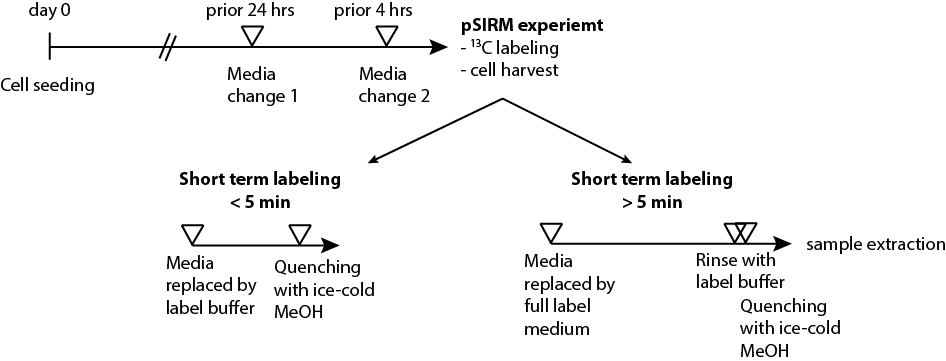
\includegraphics[width=13.14in]{images/psirm_harvest} \caption{Experimental design of a pSIRM experiment distuingishing short and long labeling with stable isotopes.}\label{fig:psirmexp}
\end{figure}

For adherent cell cultures only: Include for each experimental condition
an additional petri dish that is solely used to determine the cell count
at the time point of your harvest. This additional plate ensures a
correct determination of absolute quantities and might reduce variation
of pool sizes in the statistical analysis\footnote{Pelleting these cells
  and snap-freezing might give usefull additional samples for western
  blotting.}. Think carefully about control conditions and include cell
culture dishes that are not labeled. These dishes function as a control
for your labeling procedure and the natural abundance of isotopes.

\section{Experimental procedures}\label{experimental-procedures}

There is a slight difference in the protocols for
\protect\hyperlink{psirm:adherent}{adherent} and
\protect\hyperlink{psirm:suspension}{suspension} cells. Please read
instructions and footnotes carefully.

Short\footnote{I would rather recommend this up to 2 min of labeling}
and long term labeling procured differ only in the applied solvents
during the labeling - either label buffer
(\protect\hyperlink{washingbuffer}{LB}) only or a combination of full
label medium (LM) and label buffer (LB). Latter one is applied in order
to remove extracellular metabolites of the media. Both label buffer and
media contain the major nutrients / stable isotopes to keep the main
substrates at constant supply at all times (Table \ref{tab:solvent}).
During the application of stable isotopes longer than a few minutes
cells might sense the absence of further intermediates provided during
standard cell culture procedure and and adjust their metabolic program
accordingly.

\begin{table}[t]

\caption{\label{tab:solvent}Solvent composition of Full label medium (LM) and label buffer (BF) for a pSIRM experiment labeling with 13C-glucose.}
\centering
\begin{tabular}{llll}
\toprule
Solvent & Base & Carbon.source & Supplements\\
\midrule
Full label medium (LM) & DMEM, without glucose, glutamine, pyruvate & 13C-Glc (2.5 g/L)
12C-Gln (2 mM) & small molecules 
(inhibitor, antibiotics)\\
Label buffer (LB) & HEPES (5 mM), NaCl (140 mM), pH 7.4 & 13C-Glc (2.5 g/L)
12C-Gln (2 mM) & \\
\bottomrule
\end{tabular}
\end{table}

The quality of your data later heavily relies on the exact handling of
the cells and a \emph{consistent timing} throughout the pSIRM
experiment. Especially the step removing the LB and quenching the cells
should be a matter of a tenth of seconds rather than seconds. It is of
great value to perform the cell harvest with a second person.

\section{Protocol pSIRM}\label{protocol-psirm}

\hypertarget{psirm:adherent}{\subsection{Adherent cell
cultures}\label{psirm:adherent}}

The herein described protocols are detailed explanations how to perform
a pSIRM cell harvest for long term label application. If you want to
label for less than 2 minutes omit solely \emph{omit steps 6-8}.

Materials:

\begin{itemize}
\tightlist
\item
  Cell culture dishes, max. confluency 80 \%
\item
  Labeling media (LM) supplemented with substrates (5 ml /
  dish)\footnote{Not required for short term labeling}
\item
  Label buffer (LB) supplemented with substrates (5 ml / dish)
\item
  Ice-cold 50 \% MeOH supplemented with 2 ug/ul cinnamic acid
\item
  2x 5 ml pipette and tips\footnote{Highly recommended, makes labeling
    and harvest super quick}
\item
  Beaker
\item
  Ice
\item
  15 ml falcons (chloroform resistant)
\item
  Cell lifter
\item
  Biological waste bin next to your bench
\end{itemize}

Procedure:

\begin{enumerate}
\def\labelenumi{\arabic{enumi}.}
\tightlist
\item
  Pre-warm LB and LM in the water bath
\item
  Take a number of petri dishes (condition-wise including all biol.
  replicates)
\item
  Discard cell culture media
\item
  Carefully add \emph{long term labeling} LM OR \emph{short term
  labeling}: LB
\item
  Incubate cells on the bench or in an incubator
\item
  Discard LM (beaker)
\item
  Add immediatly 5 ml of LB
\item
  Rotate dish once in order to cover complete surface
\item
  Meanwhile 2nd person get prepared with 5 ml ice-cold MeOH
\item
  Discard LB into beaker and \emph{immediatly} 2nd person quenches with
  ice-cold MeOH
\item
  Collect cell extracts using cell lifter
\item
  Transfer cell extracts into 15 ml falcons
\item
  Store falcons on ice until further processing
\end{enumerate}

Repeat this procedure (step 6-10) for all dishes of a single condition
first. Once MeOH is added metabolic processes are interrupted and cell
extracts can be collected with the help of cell lifter without rush and
subsequently transfered to 15 ml falcon and stored on ice until further
processing (see chapter \protect\hyperlink{ccextraction_meoh}{Cell
extraction methanolic extracts}).

Determine the cell count using your additional petri dishes for each
condition.

\hypertarget{psirm:suspension}{\subsection{Supension cell
cultures}\label{psirm:suspension}}

Materials:

\begin{itemize}
\tightlist
\item
  Cell culture flasks
\item
  Labeling media (LM) supplemented with substrates
\item
  5 ml pipette and tips\footnote{Highly recommended, makes labeling and
    harvest super quick}
\item
  1 ml pipette
\item
  Beaker
\item
  paper tissues
\item
  Liquid nitrogen
\item
  15 ml falcons
\item
  1.5 ml eppendorf tubes
\item
  Biological waste bin next to your bench
\end{itemize}

Procedure:

\begin{enumerate}
\def\labelenumi{\arabic{enumi}.}
\tightlist
\item
  Pre-warm LM in the water bath
\item
  Determine the cell count of your cell suspension(s)
\item
  Take aliquots of \(10-15e+6\) cells and transfer into 15 ml falcon
\item
  Spin down cells very gently 300 g, 2 min at room temperature
\item
  Discard media into beaker
\item
  Resuspend cells gently in three-times 1 ml\footnote{To generate three
    replicates}
\item
  Incubate and keep warm
\item
  Fractionate cell supension in three eppendorf tubes (3x 1 ml each)
\item
  Spin down quickly in top-bench centrifuge\footnote{Most of the times
    30 s are already enough}
\item
  Discard media blandtly on paper tissues
\item
  Snap-freeze immediatly in liquid nitrogen
\item
  Store cells until further processing (see chapter
  \protect\hyperlink{ccextraction_susp}{Cell extraction suspension
  cells})
\end{enumerate}

The important step here to be quick is the alquotation of the cell
suspension and subsequent spin down in the table centrifuge. Suspension
cells are rather small, nevertheless \(3e+6\) cells per extract are a
good starting point for GC-MS measurements.

\section{Hints \& notes}\label{hints-notes}

\begin{itemize}
\tightlist
\item
  The only way to be reproducible and fast is to team up with a second
  person.
\item
  Keep timing consistently through the experiment.
\item
  Keep substrate concentrations constant throughout the experiment in
  all solutions.
\item
  Supplement one stable isotopic labeled substrate with all remaining
  substrates in non-labeled form.
\item
  Think about nutrient levels in your cell culture and your experimental
  conditions. Maybe you want to change things to physiological levels.
\item
  Add additional plate to each condition in order to have material for
  western blotting and others.
\item
  Check carefully the confluency of your dishes and determine seeding
  densities for different conditions.
\item
  In case of small molecule inhibitors: Try to avoid to solve them in
  DMSO - strong impact on chromatography.
\end{itemize}

\chapter{Protocols \& Procedures}\label{protocols}

\section{Materials}\label{materials}

\section{Solutions}\label{solutions}

\hypertarget{washingbuffer}{\subsection{Label
buffer}\label{washingbuffer}}

Materials:

\begin{itemize}
\tightlist
\item
  ddH2O (500 ml)
\item
  140 mM NaCl (4.1 g)
\item
  5 mM Hepes (0.569 g)
\item
  pH calibration 7.4
\end{itemize}

Procedure:

\begin{itemize}
\tightlist
\item
  Weigh the correct amounts of Hepes and NaCl
\item
  Resolve in a glas bottle with 450 ml of water
\item
  Stir carefully
\item
  Check and adjust pH
\item
  Adjust volumes to 500 ml
\end{itemize}

\subsection{MCW}\label{mcw}

Materials:

\begin{itemize}
\tightlist
\item
  Methanol
\item
  Chloroform
\item
  ddH2O
\item
  Cinnamic acid stock in MeOH (2 mg/ml): final conc. 2 ug/ml
\end{itemize}

Procedure:

\begin{itemize}
\tightlist
\item
  Mix the solvents in the ratio of volumes - Methanol:Chlorofom:Water --
  5:2:1
\item
  Supplement cinnamic acid stock 1:1000
\item
  Store at -25°C
\end{itemize}

\subsection{Alkane-Mix}\label{alkanemix}

Materials:

\begin{itemize}
\tightlist
\item
  Hexane
\item
  Alkanes: c10, c12, c15, c17, c19, c22, c28, c32, c36
\item
  Thermo mixer
\item
  Glass vials and caps
\end{itemize}

Procedure:

\begin{itemize}
\tightlist
\item
  Prepare stock solutions in hexane:
\item
  c10 - c17 (liquid): 25 ul/ml
\item
  c19 - c32: 20 mg/ml
\item
  c36: two-times 15 mg/1.5 ml
\item
  Warm up alkane stocks in thermo mixer 40°C
\item
  Prepare a text mixture in equal amounts, e.g., 50 ul each, but use
  twice the volume of c36
\item
  Mix test mixture with MSTFA: 10 ul / 1 ml MSTFA
\item
  Check alkane profile by GC-MS
\item
  If required: adjust volumes and re-test or create larger volume of
  zour mixture for aliquots
\item
  Store aiquots in glass vials, close well and store at 4°C
\item
  For usage: gently warm up glass vials at 30 C on thermo mixer for 10
  min and vortex before adding it to the MSTFA
\end{itemize}

Adjust the volumes of the alkane stocks in order to create a curve
shaped distribution of all alkanes in the chromatogram: lower
intensities for c10 and c32-36, slowly increasing intensities for the
alkanes in between.

\section{Idents \& Quant-Standards}\label{standards}

has to be written

\section{Sample Extraction}\label{SampleExtraction}

\subsection{Cell extracts}\label{cell-extracts}

Materials:

\begin{itemize}
\tightlist
\item
  cell culture dishes (10 cm), max. confluency 75\%
\item
  washing buffer (Hepes, NaCl, ph 7.4)
\item
  50\% MeOH, ice-cold
\item
  2 mg/ml cinnamic acid
\item
  chloroform
\item
  15 ml falcon tubes
\item
  cell lifter
\end{itemize}

Procedure:

\begin{itemize}
\tightlist
\item
  prepare cell culture dishes accordingly to your experimental
  conditions
\item
  discard cell culture media
\item
  add quickly 5 ml of washing buffer, discard it
\item
  add very immediately 5 ml ice-cold 50\% MeOH suppl. 2 ug/ul cinnamic
  acid
\item
  detach cells using cell lifter
\item
  collect and transfer cell extract into 15 ml falcon
\item
  store falcons until further processing on ice
\item
  add 1 ml chloroform
\item
  incube for 60 min at cold temperatures (4 C) on rotary or thermo
  shaker
\item
  centrifuge at max speed for 10 min, cold temperatures
\item
  collect polar and lipid phases into fresh falcons / tubes
\item
  dry under vacuum
\end{itemize}

In order to generate technical backups:

\begin{itemize}
\tightlist
\item
  resuspend dried extracts in 600 ul 20\% MeOH
\item
  shake at cold temperature on thermo shaker for 30 min
\item
  split volumes into equal parts in fresh eppendorf tubes
\item
  dry under vacuum
\end{itemize}

Suggested cell density: \(2-3e+6\) cells / extract.

\subsection{Tissue samples}\label{tissue-samples}

Materials:

\begin{itemize}
\tightlist
\item
  Methanol:Chloroform:Water (MCW) in ratio 5:2:1
\item
  2 mg/mg cinnamic acid in MeOH
\item
  ddH20
\item
  eppendorf tubes
\item
  tissue lyzer / pulverizer
\end{itemize}

Procedure:

\begin{itemize}
\tightlist
\item
  snap-freeze tissue samples
\item
  pulverize samples
\item
  aliquote 50 mg of tissue powder
\item
  add 1.5 ml of MCW (suppl. with cinnamic acid final conc. 2 ug/ul)
\item
  shake for 60 min on rotary shaker at cold temperature (4 C)
\item
  add 0.5 ml ddH20 for phase separation
\item
  centrifuge maximum speed, 10 min, cold temperatures
\item
  collect polar and lipid phases in fresh vessels
\item
  dry under vacuum
\end{itemize}

\subsection{Blood samples}\label{blood-samples}

Material:

\begin{itemize}
\tightlist
\item
  Methanol:Chloroform:Water (MCW) in ratio 5:2:1
\item
  2 mg/mg cinnamic acid in MeOH
\item
  ddH20
\item
  eppendorf tubes
\end{itemize}

Procedure:

\begin{itemize}
\tightlist
\item
  give 20 ul blood / sera directly into 1 ml MCW to avoid lumps
\item
  in case of lumps sonicate samples
\item
  shake samples at 4 C for 800 rpm for 60 min
\item
  add 500 ul ddH20 and vortex shortly
\item
  spin down at 4 C at max speed for 10 min
\item
  aliquote polar phase into 2-3 times 500 ul in 1.5 ml tubes
\item
  aliquote lipid phase 2 times in 100 ul lower in 1.5 ml eppi
\item
  dry in SpeedVac (35 C)
\end{itemize}

\section{Derivatisation for GC-MS}\label{Deriv}

Materials:

\begin{itemize}
\tightlist
\item
  Methoxamine (MeOx)
\item
  Pyridine (open under the hood only!)
\item
  MSTFA
\item
  Alkane mix (c10-c36) in Hexane
\item
  chromacol vials and caps (big, small)
\item
  samples: extracted and speed-vac dry for min 30 min prior procedure
\item
  quant-standards: extracted and speed-vac dry
\item
  ident-standards: extraction not required, speed-vac dry
\end{itemize}

Mixtures:

\begin{itemize}
\tightlist
\item
  Solvent 1: 40 mg MeOx in 1 ml Pyridine
\item
  Solvent 2: 10 ul Alkane mix in 1 ml MSTFA
\end{itemize}

Volumens of both solvents are shown for standard (small vol.)
procedures.

Procedure:

\begin{itemize}
\tightlist
\item
  make sure samples are completly dry (1 h speed vac)
\item
  add 20 ul (10 ul) of solvent 1 / sample
\item
  incubate on rotary shaker, 30 C, for 60 min
\item
  add 80 ul (25 ul) of solvent 2 / sample
\item
  incubaate on rotary shaker, 37 C, for 90 min
\item
  centrifuge to spin down insoluble materials
\item
  prepare aliquotes three times 28 ul or two times 15 ul (small glass
  vials)
\item
  keep on room temperature until measurement (max. 10 days)
\end{itemize}

\section{GC-MS settings}\label{gcms}

In the following paragraphs details of GC-MS settings are described in
detail. The herein described settings have been optimized for cell
extracts measured in split-mode 1:5 on the instrument Pegasus 4D-C
GC-ToF-MS in 1D mode equiped with an autosampler Gerstel MPS.

\bibliography{book.bib,packages.bib}


\end{document}
